\AtBeginSection[]
{
  \begin{frame}
    \tableofcontents[currentsection]
  \end{frame}
}

\section{Introduction}

\subsection{Julia}

\myframectr{
  \begin{itemize}
    \item High level, High performance
    \item Great C/Fortran interface
    \item Easy syntax
  \end{itemize}
}

\subsection{CUTEst}

\myframectr{
  \begin{itemize}
    \item Repository of Nonlinear Optimization problems;
    \item Provides subroutines to obtain the problem's information;
    \item Decodes the problem, compiles your code with the problem's and runs
      your main code;
    \item Widely used.
  \end{itemize}
}

\subsection{CUTEst.jl}

\myframectr{
  \begin{itemize}
    \item Easy to install;
    \item Easy to use;
    \item Easy to build in stages.
  \end{itemize}
}

\section{Why CUTEst.jl}

\subsection{CUTEst}

\begin{frame}[t,fragile]
  \ctr{CUTEst (Fortran)}
  \begin{minted}{fortran}
CALL cutest_cdimen(st, ifile, n, m)
if (m.GT.0) THEN
  STOP
ENDIF
CALL cutest_usetup(st, ifile, 7, 11, n, x, bl, bu)
CALL cutest_ufn(st, n, x, f)
\end{minted}
\end{frame}

\begin{frame}[t,fragile]
  \ctr{CUTEst.jl}
  \begin{minted}{julia}
Pkg.add("CUTEst") # Once
\end{minted}
\begin{minted}{julia}
using CUTEst

nlp = CUTEstModel("ROSENBR")
x = nlp.meta.x0

f = obj(nlp, x)
cutest_finalize(nlp)
\end{minted}
\end{frame}

\begin{frame}[t,fragile]
  \ctr{Example}
  \inputminted{julia}{src/newton.jl}
\begin{minted}{julia}
f(x) = obj(nlp, x)
g(x) = grad(nlp, x)
H(x) = hess(nlp, x)
x = newton(f, g, H, nlp.meta.x0)
\end{minted}
\end{frame}

\begin{frame}[t,fragile]
  \ctr{Example}
  \inputminted{julia}{src/newton.jl}
\begin{minted}{julia}
f(x) = ufn(nlp, x) # Familiar names
g(x) = ugr(nlp, x) # are here too
H(x) = udh(nlp, x, nlp.meta.nvar)
x = newton(f, g, H, nlp.meta.x0)
\end{minted}
\end{frame}

\subsection{Memory efficient}

\begin{frame}[t,fragile]
  \ctr{Example with inplace}
  \inputminted{julia}{src/newtoninplace.jl}
\end{frame}

\begin{frame}[t,fragile]
  \ctr{Example with inplace}
  \begin{minted}{julia}
f(x) = ufn(nlp, x)
g!(x, gx) = ugr!(nlp, x, gx)
H!(x, Hx) = udh!(nlp, x, nlp.meta.nvar, Hx)
x = newton(f, g!, H!, nlp.meta.x0)
\end{minted}
\end{frame}

\subsection{The Fortran wrapper}

\begin{frame}[t,fragile]
  \ctr{Fortran wrapper}
  \begin{minted}{julia}
io_err = Cint[0]
n = Cint[nlp.meta.nvar]
f = [0.0]
ufn(io_err, n, x, f)
\end{minted}
\end{frame}

\section{Workflow}

\myframe{
   ``... We should forget about the small efficiencies, say about 97\% of the
    time: {\bf premature optimization is the root of all evil}...'' \\
    Donald Knuth
}

\subsection{Test Driven Development}

\myframectr{
  \begin{itemize}
    \item {\it Create a failing test; Fix the test; Refactor code; Repeat.}
    \item Optimization doesn't have small building blocks;
    \item Simplest representative problem you should be able to solve;
    \item Classes of problems you should be able to solve;
    \item Selection of CUTEst problems you should be able to solve.
  \end{itemize}
}

\myframe{
  \ctr{Nonzero exit flag}
  \begin{itemize}
    \item Infinite loop;
    \item Budget limitations;
    \item Domain error.
  \end{itemize}
}

\myframe{
  \ctr{Scaling}
  \begin{itemize}
    \item Dense matrices;
    \item Inplace operations;
    \item Small efficiencies.
  \end{itemize}
}

\section{Framework}

\myframe{
  \ctr{Framework}
  \begin{itemize}
    \item CUTEst.jl
    \item NLPModels.jl
    \item Optimize.jl
  \end{itemize}
}

\subsection{NLPModels.jl}

\myframe{
  \ctr{NLPModels.jl}
\begin{center}
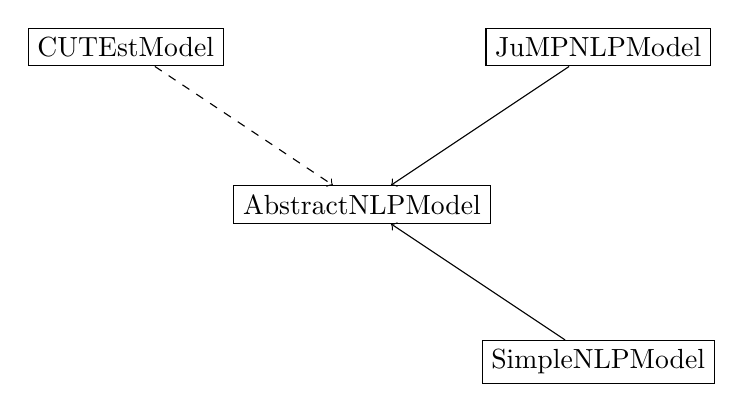
\begin{tikzpicture}
  \node[draw,rectangle] (abstract) at (0,0) {AbstractNLPModel};
  \node[draw,rectangle] (jump) at (3,2) {JuMPNLPModel};
  \node[draw,rectangle] (simple) at (3,-2) {SimpleNLPModel};
  \node[draw,rectangle] (cutest) at (-3,2) {CUTEstModel};
  \draw[->] (jump) -- (abstract);
  \draw[->] (simple) -- (abstract);
  \draw[dashed,->] (cutest) -- (abstract);
\end{tikzpicture}
\end{center}
}

\subsection{Optimize.jl}

\myframe{
  \ctr{Optimize.jl}
  \begin{itemize}
    \item Methods;
    \item Auxiliary algorithms (trust region, line search, etc.);
    \item Testing and benchmarking;
  \end{itemize}
}

\section{TRON}

\myframe{
  \ctr{A practical example}
    {\bf Newton's Method for Large Bound-Constrained Optimization
      Problems} \\
      Chih-Jen Lin and Jorge J. Moré \\
      {\it SIAM Journal on Optimization} Vol. 9, No. 4, pp. 1100-1127, 1999.
}

\myframe{
  \[ \min f(x) \quad \mbox{s. to} \quad x \in \Omega, \]
  where $\Omega$ is
  \[ \Omega = \{ x \in \mathbb{R}^n \mid \ell \leq x \leq u \}, \]
  but can be extended to
  \[ \Omega = \{ x \in \mathbb{R}^n \mid \ell \leq c_i^Tx \leq u,
  \ i \in \mathcal{I} \}. \]
}

\myframe{
  \ctr{Outline of iteration $k$}
  \begin{enumerate}
    \item Compute a model
      \[ m_k(d) = \frac{1}{2}d^TB_kd + d^Tg_k. \]
    \item Compute a gradient step $s_k = P[x_k - \alpha_kg_k] - x_k$ such that
      \[ m_k(s_k) \leq \mu_0 g_k^Ts_k, \qquad \mbox{and} \qquad
        \Vert s_k \Vert \leq \mu_1\Delta_k. \]
    \item Compute a step $d_k$ better than $s_k$, i.e., further minimizing
      $m_k$ with $\Vert d_k \Vert \leq \mu_1\Delta_k$.
    \item Update $x_k$ and $\Delta_k$ using Trust Region rules.
  \end{enumerate}
}

\myframe{
  \ctr{Minimum implementation}
  \begin{enumerate}
    \item Use $B_k = \nabla^2f(x_k)$;
    \item Use $d_k = s_k$;
    \item Trust Region is already implemented, so no need to simplify.
  \end{enumerate}
}

\myframe{
  \ctr{Simplest problems}
  \[ f(x) = \frac{1}{2}(x_1^2 + x_2^2). \]
}

\begin{frame}[t,fragile]
  \ctr{FactCheck}
  \begin{minted}{julia}
facts("Simple test") do
  x0 = [1.0; 2.0]
  f(x) = dot(x,x)/2
  g(x) = x
  H(x) = eye(2)
  nlp = SimpleNLPModel(x0, f, grad=g, hess=H)

  x, fx, dual = tron(nlp)
  @fact x --> roughly(zeros(2))
  @fact fx --> roughly(0.0)
  @fact dual --> roughly(0.0)
  ...
\end{minted}
\end{frame}

\begin{frame}[t,fragile]
  \ctr{FactCheck}
  \begin{minted}{julia}
  ...
  # Another simple test
  l = [0.5; 0.25]
  nlp = SimpleNLPModel(x0, f, grad=g, hess=H, lvar = l)

  x, fx, dual = tron(nlp)
  @fact x --> roughly(l)
  @fact fx --> roughly(f(l))
  @fact dual --> roughly(0.0)
end
\end{minted}
\end{frame}

\begin{frame}[t,fragile]
  \ctr{Implementation}
  \begin{minted}[fontsize=\small]{julia}
# Projection
P(x) = max(min(x, u), l)
# Optimality
dual(x) = norm(P(x - g(x)) - x)
# Trust region
tr = TrustRegion(SomeInitialValue)
D() = get_property(tr, :radius)
# Gradient step
s(a) = P(x - a*g(x)) - x
# Condition
q(d) = 0.5*dot(d,H(x)*d) + dot(d,g(x))
cond(s) = q(s) <= mu0*dot(g(x),s) && norm(s) <= mu1*D()
\end{minted}
\end{frame}

\begin{frame}[t,fragile]
  \ctr{Implementation}
  \begin{minted}[fontsize=\scriptsize]{julia}
sa = s(a)
if cond(s)
  while cond(a)
    a *= 2.0
    sa_new = s(a)
    sa == sa_new && break
    (sa_old, sa) = (sa, sa_new)
  end
  sa = sa_old
  a /= 2.0
else
  while !cond(a)
    a /= 2.0
    sa_old = sa
    sa = s(a)
  end
end
\end{minted}
\end{frame}

\myframe{
  \ctr{New test}
  \[ f(x) = (x_1 - 1)^2 + 100(x_2 - x_1^2)^2. \]
  \begin{itemize}
    \item Added to FactCheck;
    \item Found an error on an unvisited part of the code;
    \item Code coverage;
    \item With bounds $\rightarrow$ another test.
  \end{itemize}
}

\begin{frame}[t,fragile]
  \ctr{Limits}
  \begin{minted}{julia}
f(x) = begin sleep(0.1); sum(exp(x)) end
g(x) = begin sleep(0.1); exp(x) end
H(x) = begin sleep(0.1); spdiagm(exp(x), 0, 10, 10) end
x0 = 10*ones(10)
\end{minted}
\end{frame}

\myframe{
  \ctr{New test}
  \[ f(x) = \frac{1}{2}(x-r)^TQ^T\Lambda Q(x-r) + 1, \]
  where
  \begin{itemize}
    \item $r = (1,\dots,1)^T$;
    \item $Q$ is an orthogonal matrix;
    \item $\Lambda = \mbox{diag}(10^{-4}, \dots, 1)^T$
  \end{itemize}
}

\myframe{
  \ctr{New test}
  \[ \min \ f(x) = \frac{1}{2}x^TBx + g^Tx, \quad \mbox{s. to} \quad
    \ell \leq x \leq u, \]
  where
  \begin{itemize}
    \item $B = Q^T\Lambda Q > 0$.
    \item Build solution and choose $g$
  \end{itemize}
}

\subsection{Thanks}
